\documentclass{article}

\usepackage{color,amsmath,amssymb,graphicx,fancyhdr,amsfonts,amsthm,verbatim,bbold,environ}
\usepackage{hyperref}
\usepackage{mkolar_definitions}
\usepackage{multirow}
\usepackage{diagbox}
\usepackage{longtable,booktabs}
\usepackage[left=2cm,top=2cm,right=2cm]{geometry}
% \numberwithin{algorithm}{section}

\newcommand{\tightlist}{%
  \setlength{\itemsep}{0pt}\setlength{\parskip}{0pt}}


%%%%%%%%%%%%%%%%%%%%%%%%%%%%%
\newcommand{\tta}{\theta}
\newcommand{\lag}{\left\langle}
\newcommand{\rag}{\right\rangle}
\newcommand{\lnorm}{\left\|}
\newcommand{\rnorm}{\right\|}
%%%%%%%%%%%%%%%%%%%%%%%%%%%%%

\usepackage[ruled,lined,boxed,linesnumbered]{algorithm2e}


\title{EI338 Computer System Engineering Homework 5}
\author{Zhou Litao 518030910407 F1803016}
\date{\today , Fall Semester}
\begin{document}
\maketitle

%%%%%%%%%%%%%%%%%%%%%%%%%%%%%%%%%%%%%%%%%%
%%%%%%%%%%%%%                 %%%%%%%%%%%%
%%%%%%%%%%%%%    EXERCISE 1   %%%%%%%%%%%%
%%%%%%%%%%%%%                 %%%%%%%%%%%%
%%%%%%%%%%%%%%%%%%%%%%%%%%%%%%%%%%%%%%%%%%
\begin{exercise}[]{Figure~\ref{fig3} shows a flow network on which an $s$-$t$ flow has been computed. The capacity of each edge appears as a label next to the edge, and the numbers in boxes give the amount of flow sent on each edge. Edges without boxed numbers have no flow being sent on them.

    \begin{enumerate}
        \item What is the value of this flow? Is this a maximum $(s, t)$ flow in this graph? If not, calculate the value of the maximum flow.
        \item Find a minimum $s$-$t$ cut in the flow network. Calculate its capacity.
    \end{enumerate}
    
    \begin{figure}[h]
        \centering
        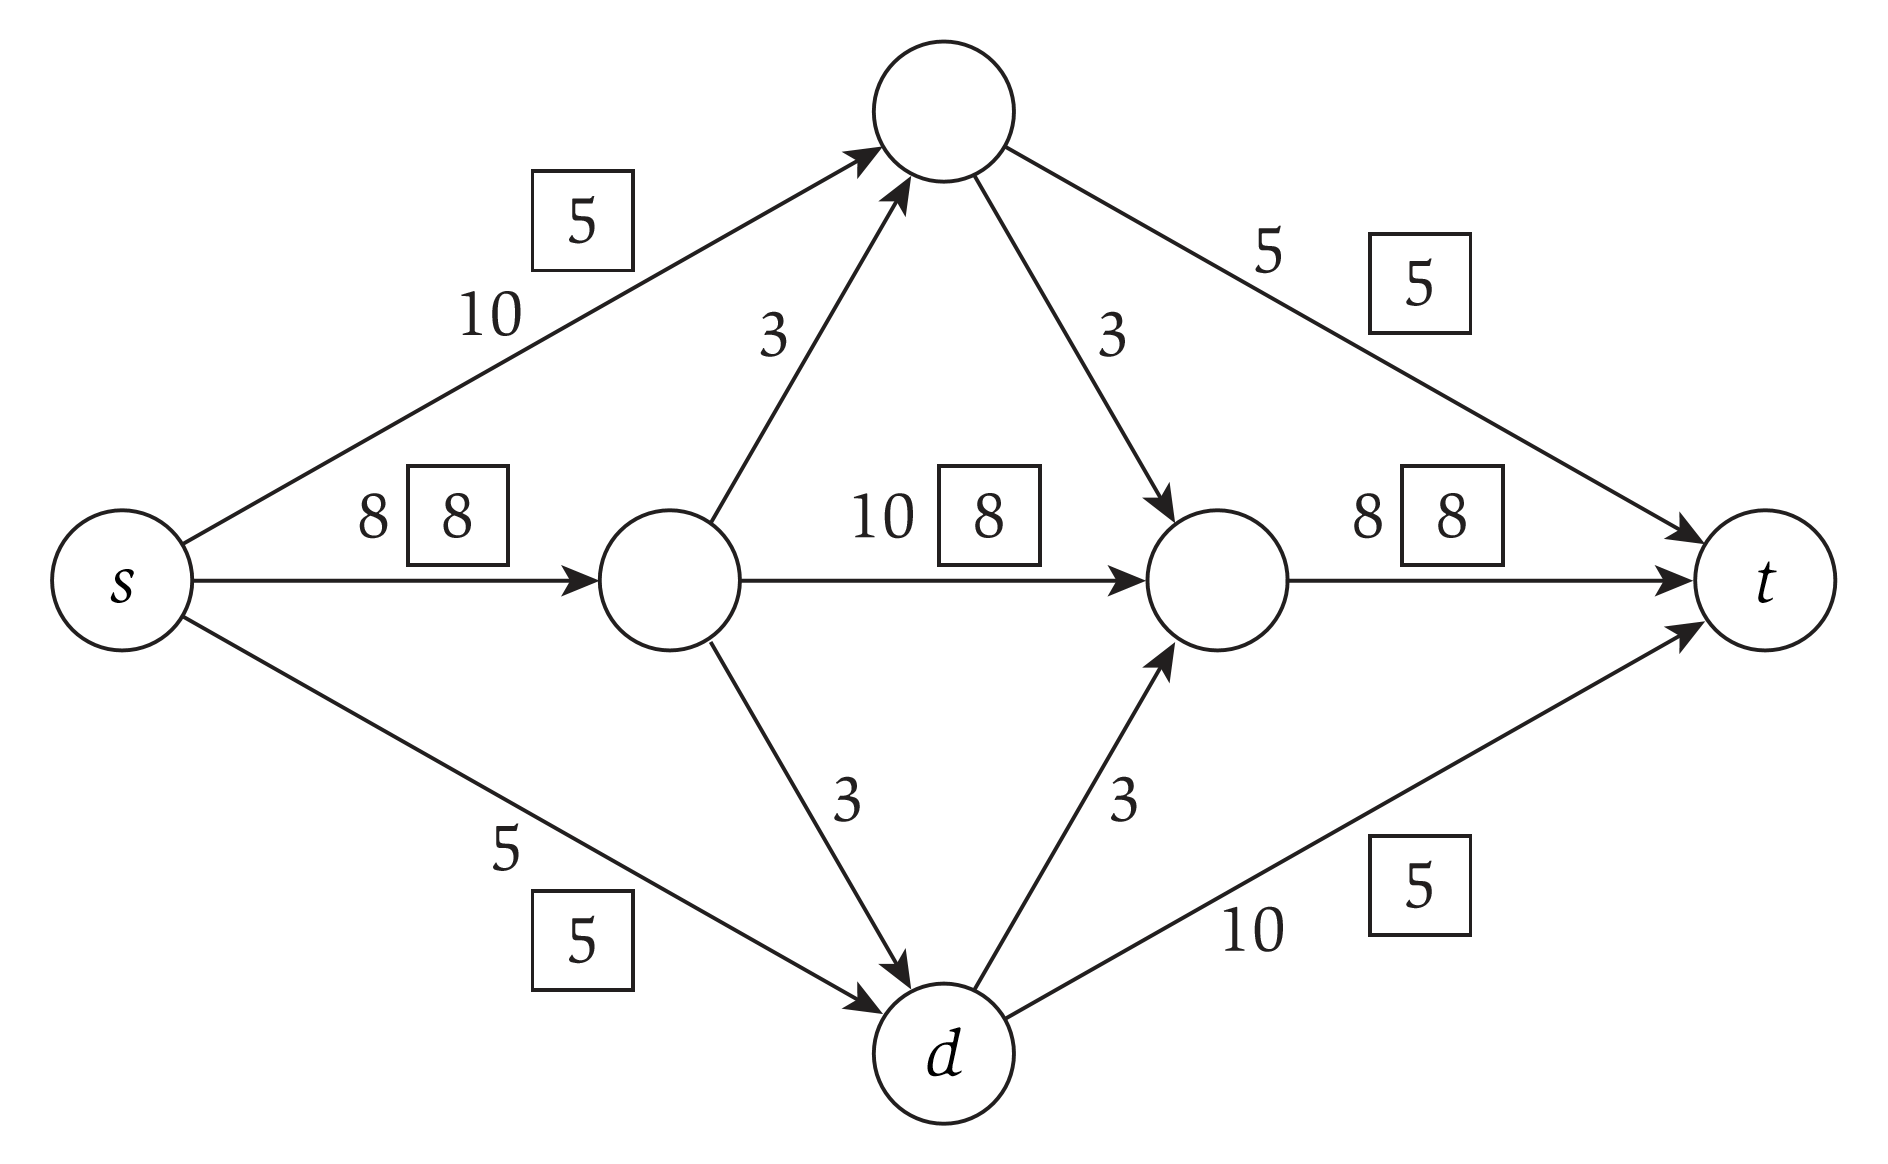
\includegraphics[width=0.5\linewidth]{img/fig3.png}
        \caption{A flow network.}
        \label{fig3}
    \end{figure}
    }
  \begin{solution}
  \par{~}
  \begin{enumerate}
    \item {
      The value of this flow is $5+8+5=18$. It is not a maximum flow. The maxmimum flow is 21, depicted in \ref{fig4}.
      \begin{figure}[h]
        \centering
        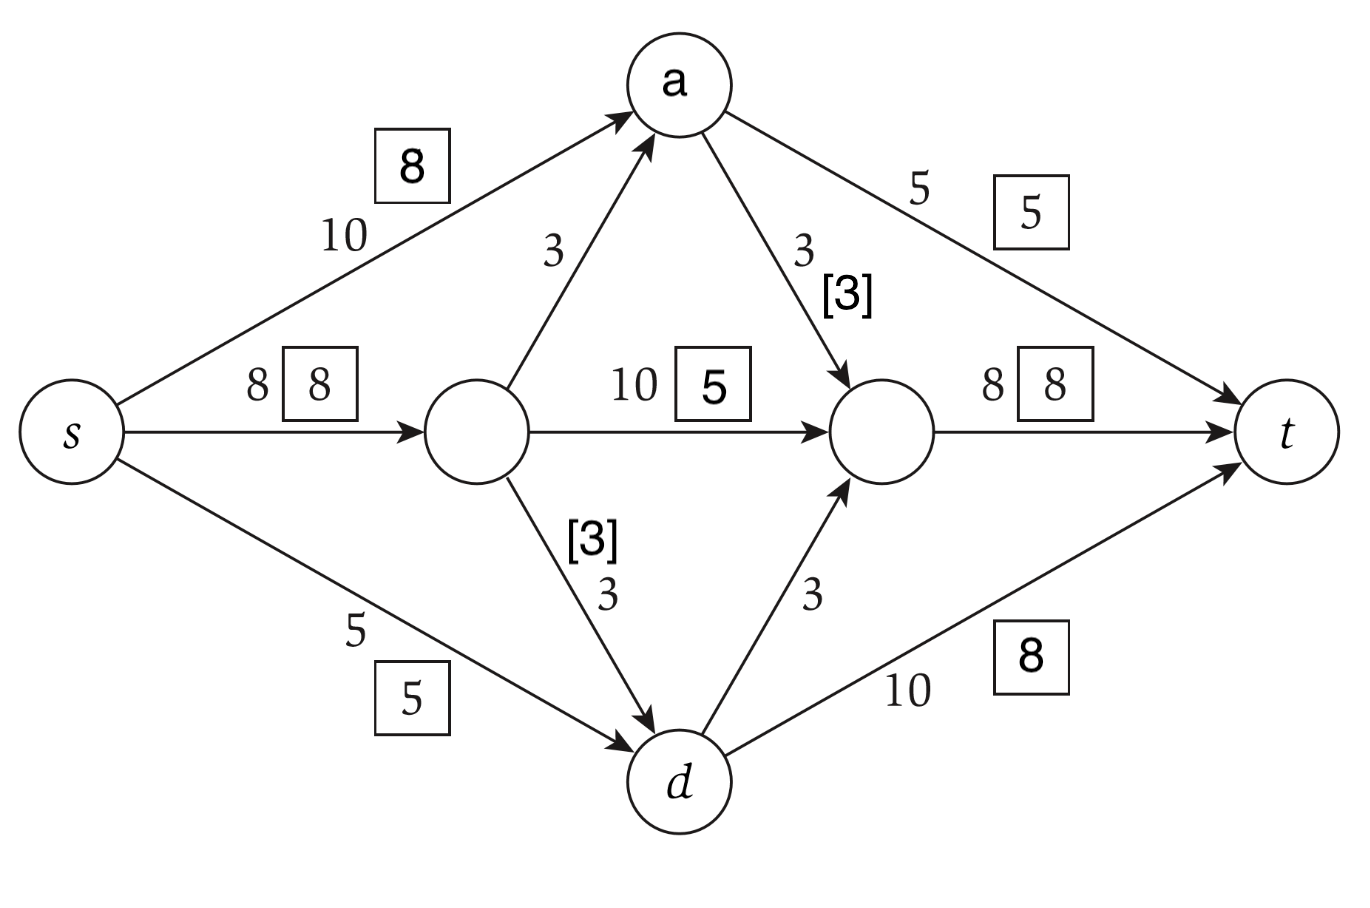
\includegraphics[width=0.5\linewidth]{img/ex5-1.png}
        \caption{My flow network.}
        \label{fig4}
    \end{figure}
    }
    \item {
      The minimum s-t cut is composed of $\{s, a\}$ and the other nodes. Its capacity is $5+8+5+3=21$
    }
  \end{enumerate}
  \end{solution}
  \label{ex1}
\end{exercise}

%%%%%%%%%%%%%%%%%%%%%%%%%%%%%%%%%%%%%%%%%%
%%%%%%%%%%%%%                 %%%%%%%%%%%%
%%%%%%%%%%%%%    EXERCISE 2   %%%%%%%%%%%%
%%%%%%%%%%%%%                 %%%%%%%%%%%%
%%%%%%%%%%%%%%%%%%%%%%%%%%%%%%%%%%%%%%%%%%
\begin{exercise}[]{We define the \textit{Escape Problem} as follows. We are given a directed graph $G=(V,E)$ (picture a network of roads). A certain collection of nodes $X \subset V$ are designated as \textit{populated nodes}, and a certain other collections $S \subset V$ are designated as \textit{safe nodes}. $X$ and $S$ are disjoint. In case of an emergency, we want evacuation routes from the populated nodes to the safe nodes. A set of evacuation routes is defined as a set of paths in $G$ so that (i) each node in $X$ is the head of one path, (ii) the last node on each path lies in S, and (iii) the paths do not share any edges. Such a set of paths gives a way for the occupants of the populated nodes to "escape" to safe nodes, without overly congesting any edge in $G$.

    \begin{enumerate}
        \item Given $G$, $X$ and $S$, show how to decide in polynomial time whether such a set of evacuation routes exists.
        \item Suppose we have exactly the same problem as in (a), but we want to enforce an even stronger version of the "no congestion" condition (iii). Thus we change (iii) to say "the paths do not share any nodes". 
        
        With this new condition, show how to decide in polynomial time whether such a set of evacuation routes exists. 
        
        Also, provide an example with the same $G$, $X$ and $S$, in which the answer is yes to the question in (a) but no to the question in (b).
    \end{enumerate}
    }
  \begin{solution}
  \par{~}
  \begin{enumerate}
    \item Based on the graph given in the problem, let all edges have a unit capacity. Then, add a starting node $s$ and add an edge with unit capacity from $s$ to every node in $X$. Also, add a end ending node $t$ and connect all the nodes in $S$ to it with unit capacity. With the flow graph constructed, use Ford-Fulkerson algorithm to find the maximum flow, which runs in polynomial time given all the capacities are 1. If the maximum flow is $|X|$, such a set of evacuation routes can be found. Otherwise, there exists no such non-intersecting evacuation routes.
    \item For every node that are neither populated nodes nor safe nodes, expand it into two nodes, with a unit capacity between them. Then we can make sure that the node in the original graph will be assigned a unique group to pass by.
    
    An example is presented below in \ref{fig:ans}\begin{figure}[h]
      \centering
      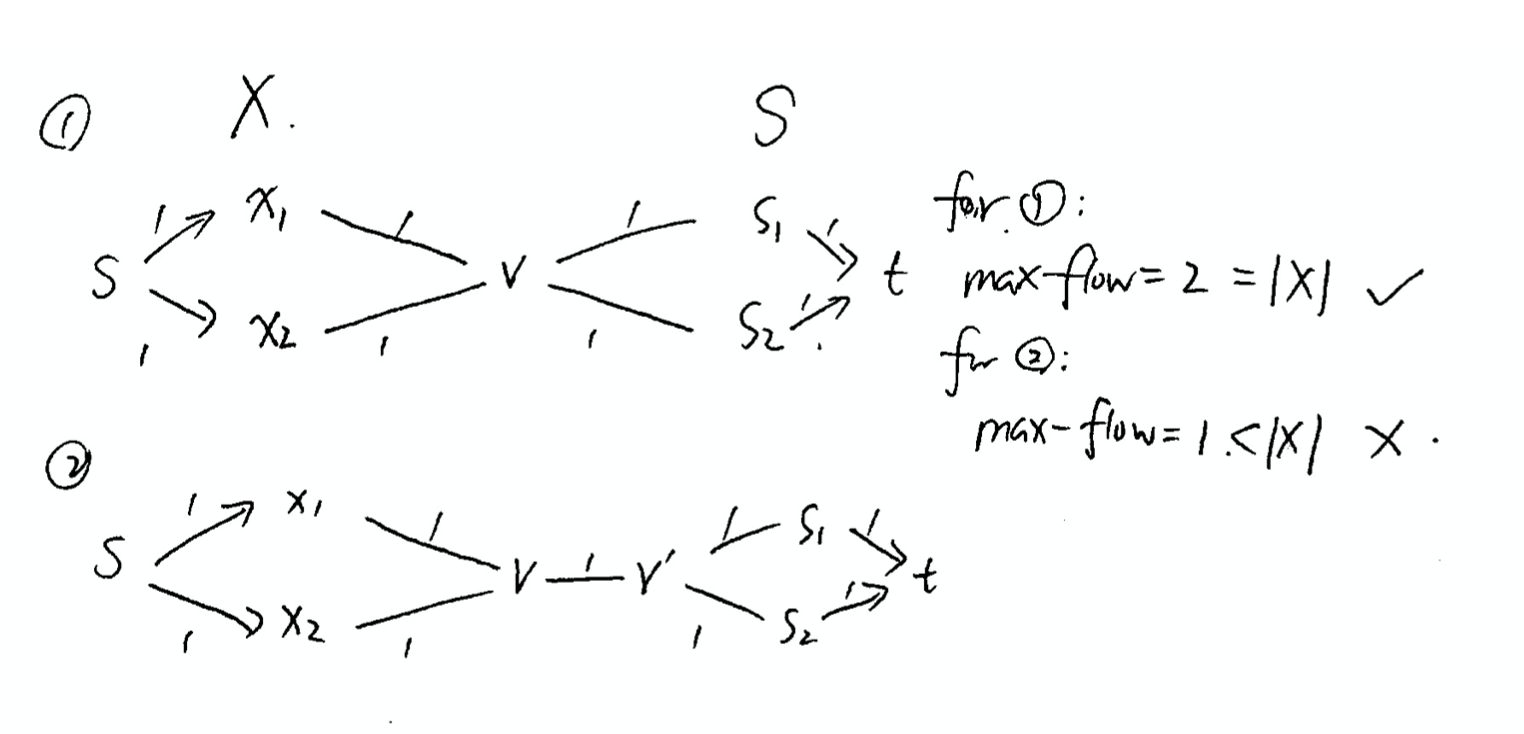
\includegraphics[width=0.5\linewidth]{img/ex5-2.png}
      \caption{An example for Problem 2.}
      \label{fig:ans}
  \end{figure}
  \end{enumerate}
  \end{solution}
  \label{ex2}
\end{exercise}


%%%%%%%%%%%%%%%%%%%%%%%%%%%%%%%%%%%%%%%%%%
%%%%%%%%%%%%%                 %%%%%%%%%%%%
%%%%%%%%%%%%%    EXERCISE 3   %%%%%%%%%%%%
%%%%%%%%%%%%%                 %%%%%%%%%%%%
%%%%%%%%%%%%%%%%%%%%%%%%%%%%%%%%%%%%%%%%%%
\begin{exercise}[]{Suppose there are n people living in a cooperative apartment. Over the next $n$ nights, each of you is supposed to cook dinner for the co-op exactly once, so that someone cooks on each of the nights.

    Of course, everyone has scheduling conflicts with some of the nights, so deciding who should cook on which night becomes a tricky task. For concreteness, let's label the people $\{p_1, ..., p_n\}$ and the nights $\{d_1, ..., d_n\}$. For person $p_i$, there's a set of nights $S_i \subset \{d_1, ..., d_n\}$ when they are able to cook.
    
    A feasible dinner schedule is an assignment of each person in the co-op to a different night, so that each person cooks on exactly one night, and there is someone cooking on each night. If $p_i$ cooks on night $d_j$, then $d_j \in S_i$.
    
    \begin{enumerate}
        \item Describe a bipartite graph $G$ so that $G$ has a perfect matching if and only if there is a feasible dinner schedule for the co-op.
        \item There is a schedule constructed by your friend. Unfortunately, when you look at the schedule she created, you notice a big problem. $n-2$ of the people at the co-op are assigned to different nights on which they are available: no problem there. But for the other two people, $p_i$ and $p_j$, and the other two days, $d_k$ and $d_l$, you discover that she has accidentally assigned both $p_i$ and $p_j$ to cook on night $d_k$, and assigned no one to cook on night $d_l$.
        
        You want to fix this mistake without having to recompute everything from scratch. Show that it's possible, using the "almost correct" schedule, to decide in only $O(n^2)$ time whether there exists a feasible dinner schedule for the co-op.
    \end{enumerate}   }
  \begin{solution}
  \par{~}
  \begin{enumerate}
    \item We can construct a G with $V=P\cup D$ and $E = \{(p_i,d_j)|d_j \in S_i\}$. The graph is divided into $P$ and $D$, with $|P|=|D|=n$. There is a feasible dinner schedule if and only if there is a perfect matching in G.
    \item We can solve the problem by using a max-flow model. First, construct the graph described in 1, then remove all the correctly assigned $(p_x,d_x)$ edges, and add a reverse edge $(d_x,p_x)$ in the graph. Then let $(p_i,d_k)$ also be reversed. To correct the mistake, we just need to start from $p_j$ and check whether there exists a simple path to $d_l$. If the path exists, then there exists a feasible dinner schedule by reversing the edges along the path. Then all the backward edges can form a perfect matching.
    
    The construction of the graph takes $O(n^2)$ time and the finding of simple path takes $O(|E|)<O(n^2)$ time. Therefore the overall algorithm runs in $O(n^2)$ time.
  \end{enumerate}
  
  \end{solution}
  \label{ex3}
\end{exercise}

%%%%%%%%%%%%%%%%%%%%%%%%%%%%%%%%%%%%%%%%%%
%%%%%%%%%%%%%                 %%%%%%%%%%%%
%%%%%%%%%%%%%    EXERCISE 4   %%%%%%%%%%%%
%%%%%%%%%%%%%                 %%%%%%%%%%%%
%%%%%%%%%%%%%%%%%%%%%%%%%%%%%%%%%%%%%%%%%%
\begin{exercise}[]{Recall that in the standard network flow problem we required that the for each vertex $v$ (excluding the source s and sink t) the sum of the flow into that vertex is equal to the sum of flow out of that vertex. Suppose that we replace this conservation constraint with a taxation constraint. In particular, suppose each vertex represents a country and that each country $v \notin  \{s, t\}$ has an associated tax-rate $0 < t_v < 1$ meaning that country $v$ will keep
    $t_v$ fraction of the goods flowing through node $v$. Given a flow network $G = (V, E)$ with maximum capacities $c(e)$ on each edge $e \in V$ and tax rates $t_v$ for each node $v \notin {s, t}$ our goal is to find the maximum amount of goods that can be transported from $s$ to $t$ under these taxation constraints. Write down your algorithm to solve this problem. You should explain why your algorithm is correct. }
  \begin{solution}
  \par{~}
  % The problem can be solved in a similar pattern like the max-flow problem. First construct a graph $G_f$ with the same vertex set and edge value as the flow value of the original flow graph. As we proceed in finding the flow, maintain the property that for every edge $e=(u,v)$ in $G$, there exists a forward edge and a backward edge in $G(f)$. $f(e)$ represents the flow that has been occupied and $f(e')$ is the backward edge with value $c(e) - f(e)$.

  % Then we repeat the following process, every time we will try to find a simple path in $G_f$. However, when determining the bottleneck, we should take the taxation discount into consideration, i.e. we need to make sure that for every edge in the path $\prod_{i=1}^{k}t_i b \le f(e)$, where $t_1,\ldots,t_k$ is the discount value of the predecessor nodes in the path and $b$ is the bottleneck value to be determined. With the bottleneck calculating function defined, the augment path finding algorithm can be described as follows in Algorithm \ref{Alg_Aug}.

  % \begin{algorithm}[H]
  %   \KwIn{The current flow $f$, a feasible path in $G_f$ $P$}
  %   \KwOut{flow $f$ after augmenting}

  %   \BlankLine
  %   \caption{Augmenting}\label{Alg_Aug}

  %   $b=$\texttt{bottleneck}$(P,f)$\;
  %   \ForEach{$(u,v)\in P$}{
  %     \eIf{$e=(u,v)$ is a forward edge}{
  %       $f(e) = f(e) + \prod t_i b$
  %     }{
  %       let $e'=(v,u)$\;
  %       $f(e) = f(e) - \prod t_i b$
  %     }
  %   }
  %   \Return{f}
  % \end{algorithm}

  % \begin{algorithm}[H]
  %   \KwOut{maximum flow $f$}

  %   \BlankLine
  %   \caption{Max Flow}\label{Alg_flow}
  %   Initialize all $f(e) = 0$ for edges $e$ in $G$ \;
  %   \While{ there exists a simple path $P$ in $G_f$}{
  %     $f' =$\texttt{augment}$(f,P)$\;
  %     update $f$ to $f'$\;
  %     update $G_f$ to $G_{f'}$
  %   }
  %   \Return{f}
  % \end{algorithm}
  % By iterating the above augmenting algorithm until no more simple paths can be found in $G_f$ from $s$ to $t$, we can get the maximum flow in this problem.

  % To show that our algorithm is correct, first note that after augmenting, $f'$ is still a valid flow in $G$, since our bottleneck function has been designed to satisfy the taxation constraints. Then we note that $v(f') = v(f) + \prod t_i bottleneck(P,f)$, where $t_i$s are the passing nodes on path $P$, since $t_i > 0$ for every $i$ and $bottleneck(P,f)>0$, we have that $v(f')>v(f)$.
  
  % When the algorithm terminates, it follows that no more simple path can be found in $G_f$. Since the reachability of $G_f$ indicates the possibility to increase flow, we can conclude that the maximum flow is found on termination of the algorithm.


    The problem can be formulated as a linear programming problem and be solved through simplex algorithm.

    Let all the nodes excluding $s$ and $t$ be given index $i=1,\ldots,n-1$, and $s$ be given index $0$, $t$ be given index $n$. Let $c_{ij}$ denote the capacity from node $i$ to $j$ and $f_{ij}$ denote the actual flow from $i$ to $j$ used in the final solution. For every flow, we have that
    \begin{equation}
      0 \le f_{ij} \le c_{ij}, \forall i, j
    \end{equation}
    For every node, we have that
    \begin{equation}
      t_k  \sum_{i=0}^{n} f_{ik} = \sum_{j=0}^n f_{kj}, \forall k=1,\ldots,n-1
    \end{equation}
    The maximum amount of goods that can be transported can be defined as $\sum_{i=0}^{n-1} f_{in}$. i.e. the flow into $t$. We have formulated a linear programming model as follows.
    \begin{equation}
      \begin{aligned}
        \max_{f_{ij}, f'_{ij}}  & \sum_{i=0}^{n-1} f_{in} \\
        \text{s.t. } f_{ij} &\ge 0, \forall i,j = 1 \ldots n\\
        f'_{ij} &\ge 0, \forall i,j = 1 \ldots n \\
        f'_{ij} &= c_{ij} - f_{ij}, \forall i,j = 1 \ldots n\\
         \sum_{j=0}^n f_{kj} -  t_k \sum_{i=0}^{n} f_{ik} &= 0, \forall k = 1 \ldots n-1
      \end{aligned}
      \label{eqn}
    \end{equation}
    The problem has already been transformed into a slack problem $P$ in Problem \ref{eqn}, with basis variables $f'_{ij}$. A trivial initial solution is to assign all $f_{ij}$ to be 0.
    We can use the simplex algorithm to solve this problem $P$. The algorithm is described as follows. Every time we run the algorithm, the solution will be improved, until the solution converges.


    For sake of simplicity in expression, we denote $c$ to be the coefficient vector for the objective function and $A$ to be the coefficient matrix for equality constraints.
    
\begin{algorithm}[H]
  \setcounter{algocf}{1}
  \caption{Simplex Algorithm}
  \label{algo2}
  
  \AlgoDisplayBlockMarkers\AlgoDisplayGroupMarkers\SetAlgoBlockMarkers{ \{}{ \}\ }%
  \SetAlgoNoEnd\SetAlgoNoLine
  
  \SetKwInOut{Input}{Input}\SetKwInOut{Output}{Output}
  \Input{Linear program (P) and feasible basis $B$}
  \Output{An optimal solution for (P) or a certificate proving that (P) is unbounded }
  Rewrite (P) so that it is in canonical form for the basis $B$\\
  Let $\vec{x}$ be the basic feasible solution for $B$\\
  \If{$\vec{c_N} \le \vec{0}$}{
  {\bf stop}\\
  ($\vec{x}$ is optimal)
  }
  Select $k \in N$ such that $c_k > 0$\\
  \If{$A_k \le \vec{0}$}{
  {\bf stop}\\
  ((P) is unbounded)
  }
  Let \emph{r} be any index \emph{i} where the following minimum is attained:
  \begin{equation}
  t = \operatorname{min}\left\{\frac{b_i}{A_{i,k}}:A_{i,k} > 0\right\}
  \end{equation}
  \\
  Let $\iota$ be the $r^{th}$ basis element\\
  Set $B:=B\cup\{k\}$\textbackslash$\{\iota\}$\\
  Go to step 1
  \end{algorithm}
  \end{solution}
  \label{ex4}
\end{exercise}


\end{document}